\documentclass{article}
\usepackage[UKenglish]{babel}

\usepackage{graphicx}
\usepackage{booktabs}
\usepackage{tabularX}
\usepackage{multirow}
\usepackage{amsmath}
\usepackage{natbib}
\usepackage{color}

%\usepackage[paperwidth=15.75cm, paperheight=5cm, margin=0cm]{geometry}
\usepackage[paperwidth=174mm, paperheight=225mm, margin=0cm]{geometry}
%\renewcommand{\familydefault}{\sfdefault}
\usepackage{fontspec}
\setmainfont{Arial}
\setlength\parindent{0pt}

\begin{document}
\hspace{-0.5em}
\begin{tabular}{l@{\hspace{4mm}}l}
  \large{A} &\large{B}\\
  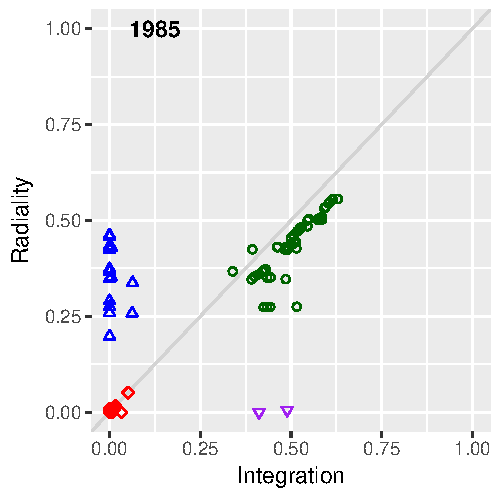
\includegraphics{Figure6a.pdf}&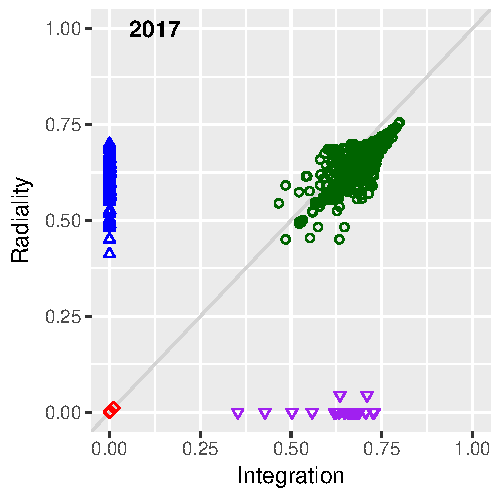
\includegraphics{Figure6b.pdf}\\
  \large{C} \\
  \multicolumn{2}{c}{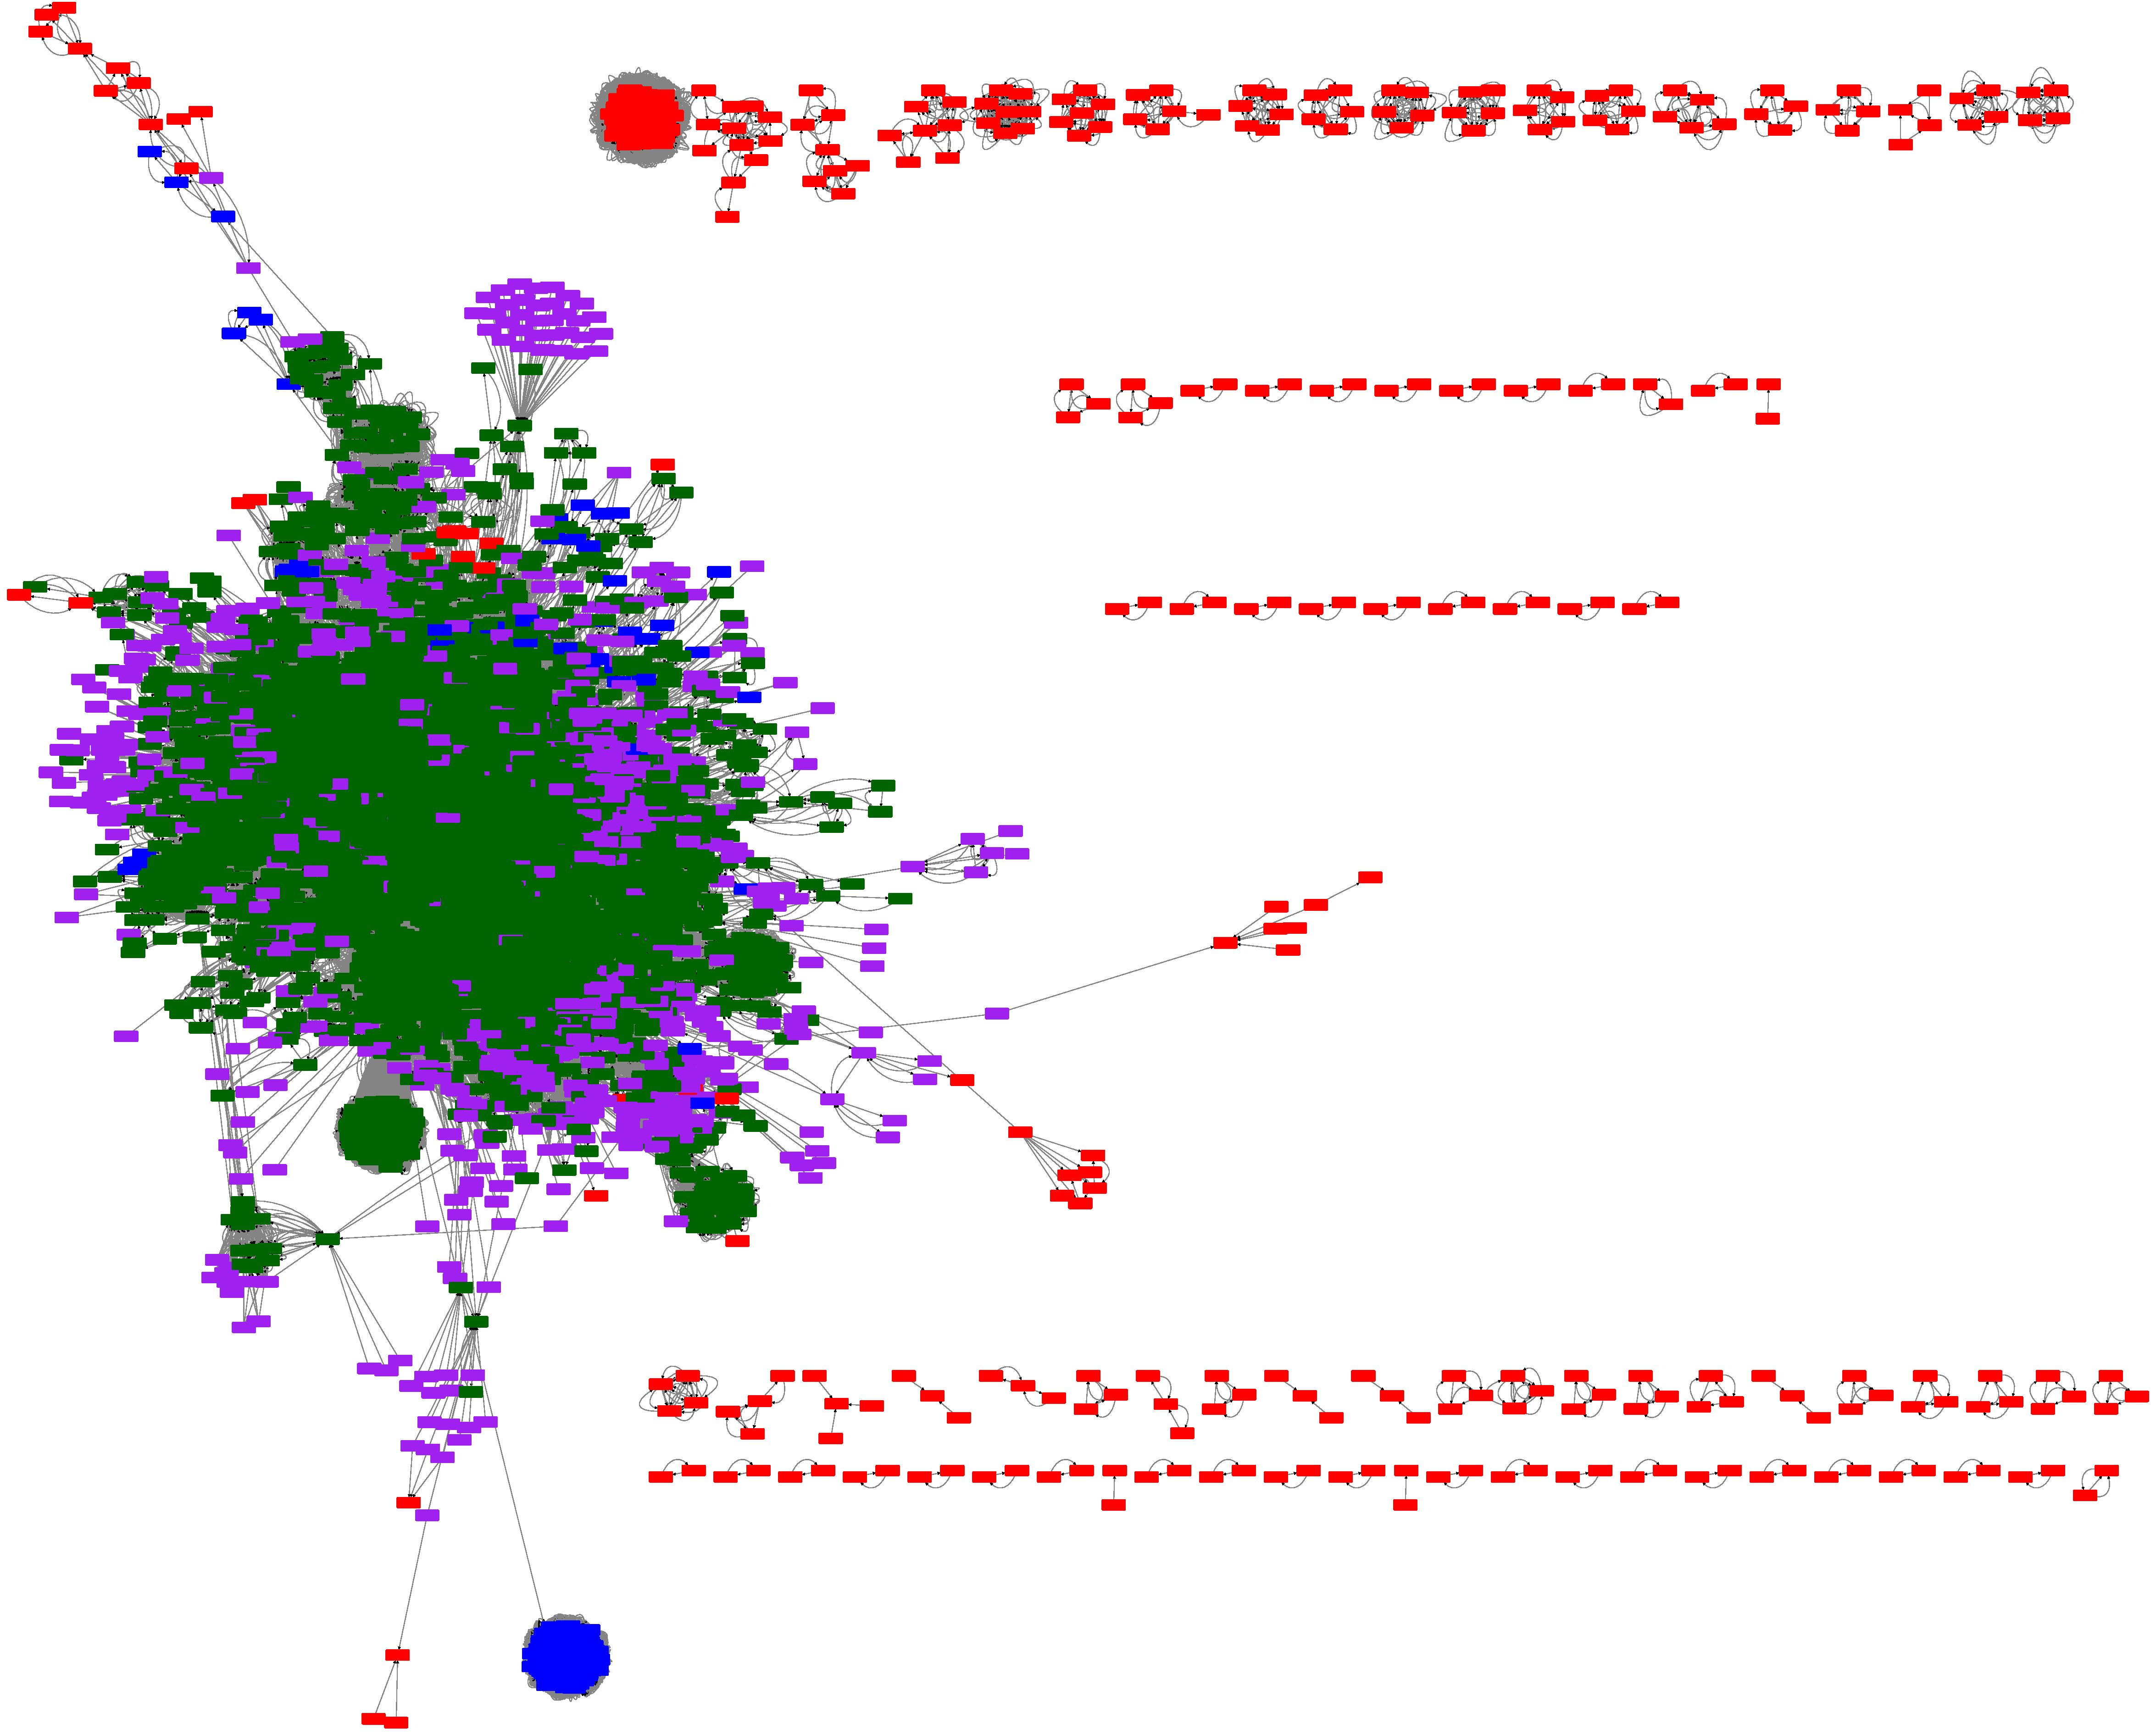
\includegraphics[width=0.9\textwidth]{2017RadIntNewRedone.jpeg}}
\end{tabular}
\end{document}

\hspace{-2em}
\begin{tabular}{l@{\hspace{4mm}}r}
  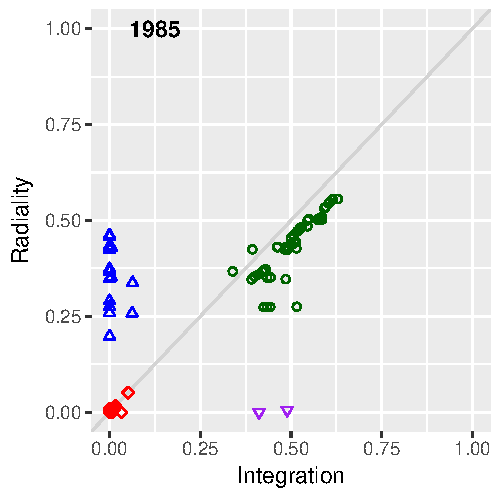
\includegraphics{Figure6a.pdf}&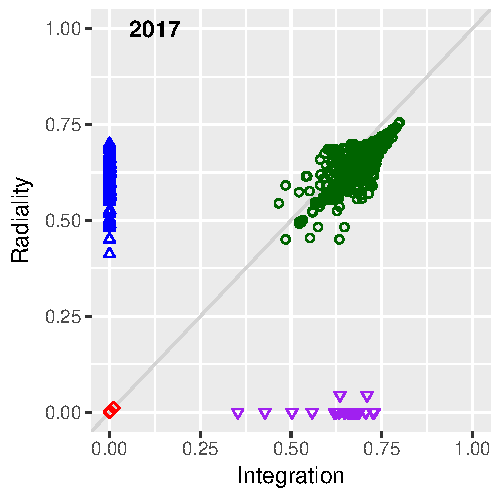
\includegraphics{Figure6b.pdf}
\end{tabular}
